\documentclass[12pt]{article}
\usepackage[margin=1in]{geometry}
\usepackage{listings}
\usepackage{graphicx}
\usepackage{float}
\usepackage{color} %red, green, blue, yellow, cyan, magenta, black, white
\definecolor{mygreen}{RGB}{28,172,0} % color values Red, Green, Blue
\definecolor{mylilas}{RGB}{170,55,241}

\setlength{\parskip}{1em}

\lstset{language=Matlab,%
    %basicstyle=\color{red},
    breaklines=true,%
    morekeywords={matlab2tikz},
    keywordstyle=\color{blue},%
    morekeywords=[2]{1}, keywordstyle=[2]{\color{black}},
    identifierstyle=\color{black},%
    stringstyle=\color{mylilas},
    commentstyle=\color{mygreen},%
    showstringspaces=false,%without this there will be a symbol in the places where there is a space
    numbers=left,%
    numberstyle={\tiny \color{black}},% size of the numbers
    numbersep=9pt, % this defines how far the numbers are from the text
    emph=[1]{for,end,break},emphstyle=[1]\color{red}, %some words to emphasise
    %emph=[2]{word1,word2}, emphstyle=[2]{style},    
}


\title{Assignment 1, COMP4702}
\author{Roy Portas}
\date{\today}

\begin{document}

\begin{titlepage}
    \maketitle
\end{titlepage}

\section*{Question 1.2}

The first column of the data is the date, the second column appears to be a
unique ID for each entry.

The third column contains numbers between 25 and 30, this is possibly a
temperature in degrees. The values also change gradually which seems correct
for the given time intervals

The fourth column contains numbers between 26 and around 50000. If this is
plotted against the ID field, it produces a line.

The fifth column contains numbers between 7.3 and 8.3, with a mean of 7.846 and
a standard StdDev of 0.142. This suggests that the value doesn't change much.

It could possibly be weather data, containing temperature, humidity, etc.

\section*{Question 1.6}

\lstinputlisting[language=Matlab]{../../pracs/week2/q6.m}

\section*{Question 2.1}

\begin{figure}[H]
    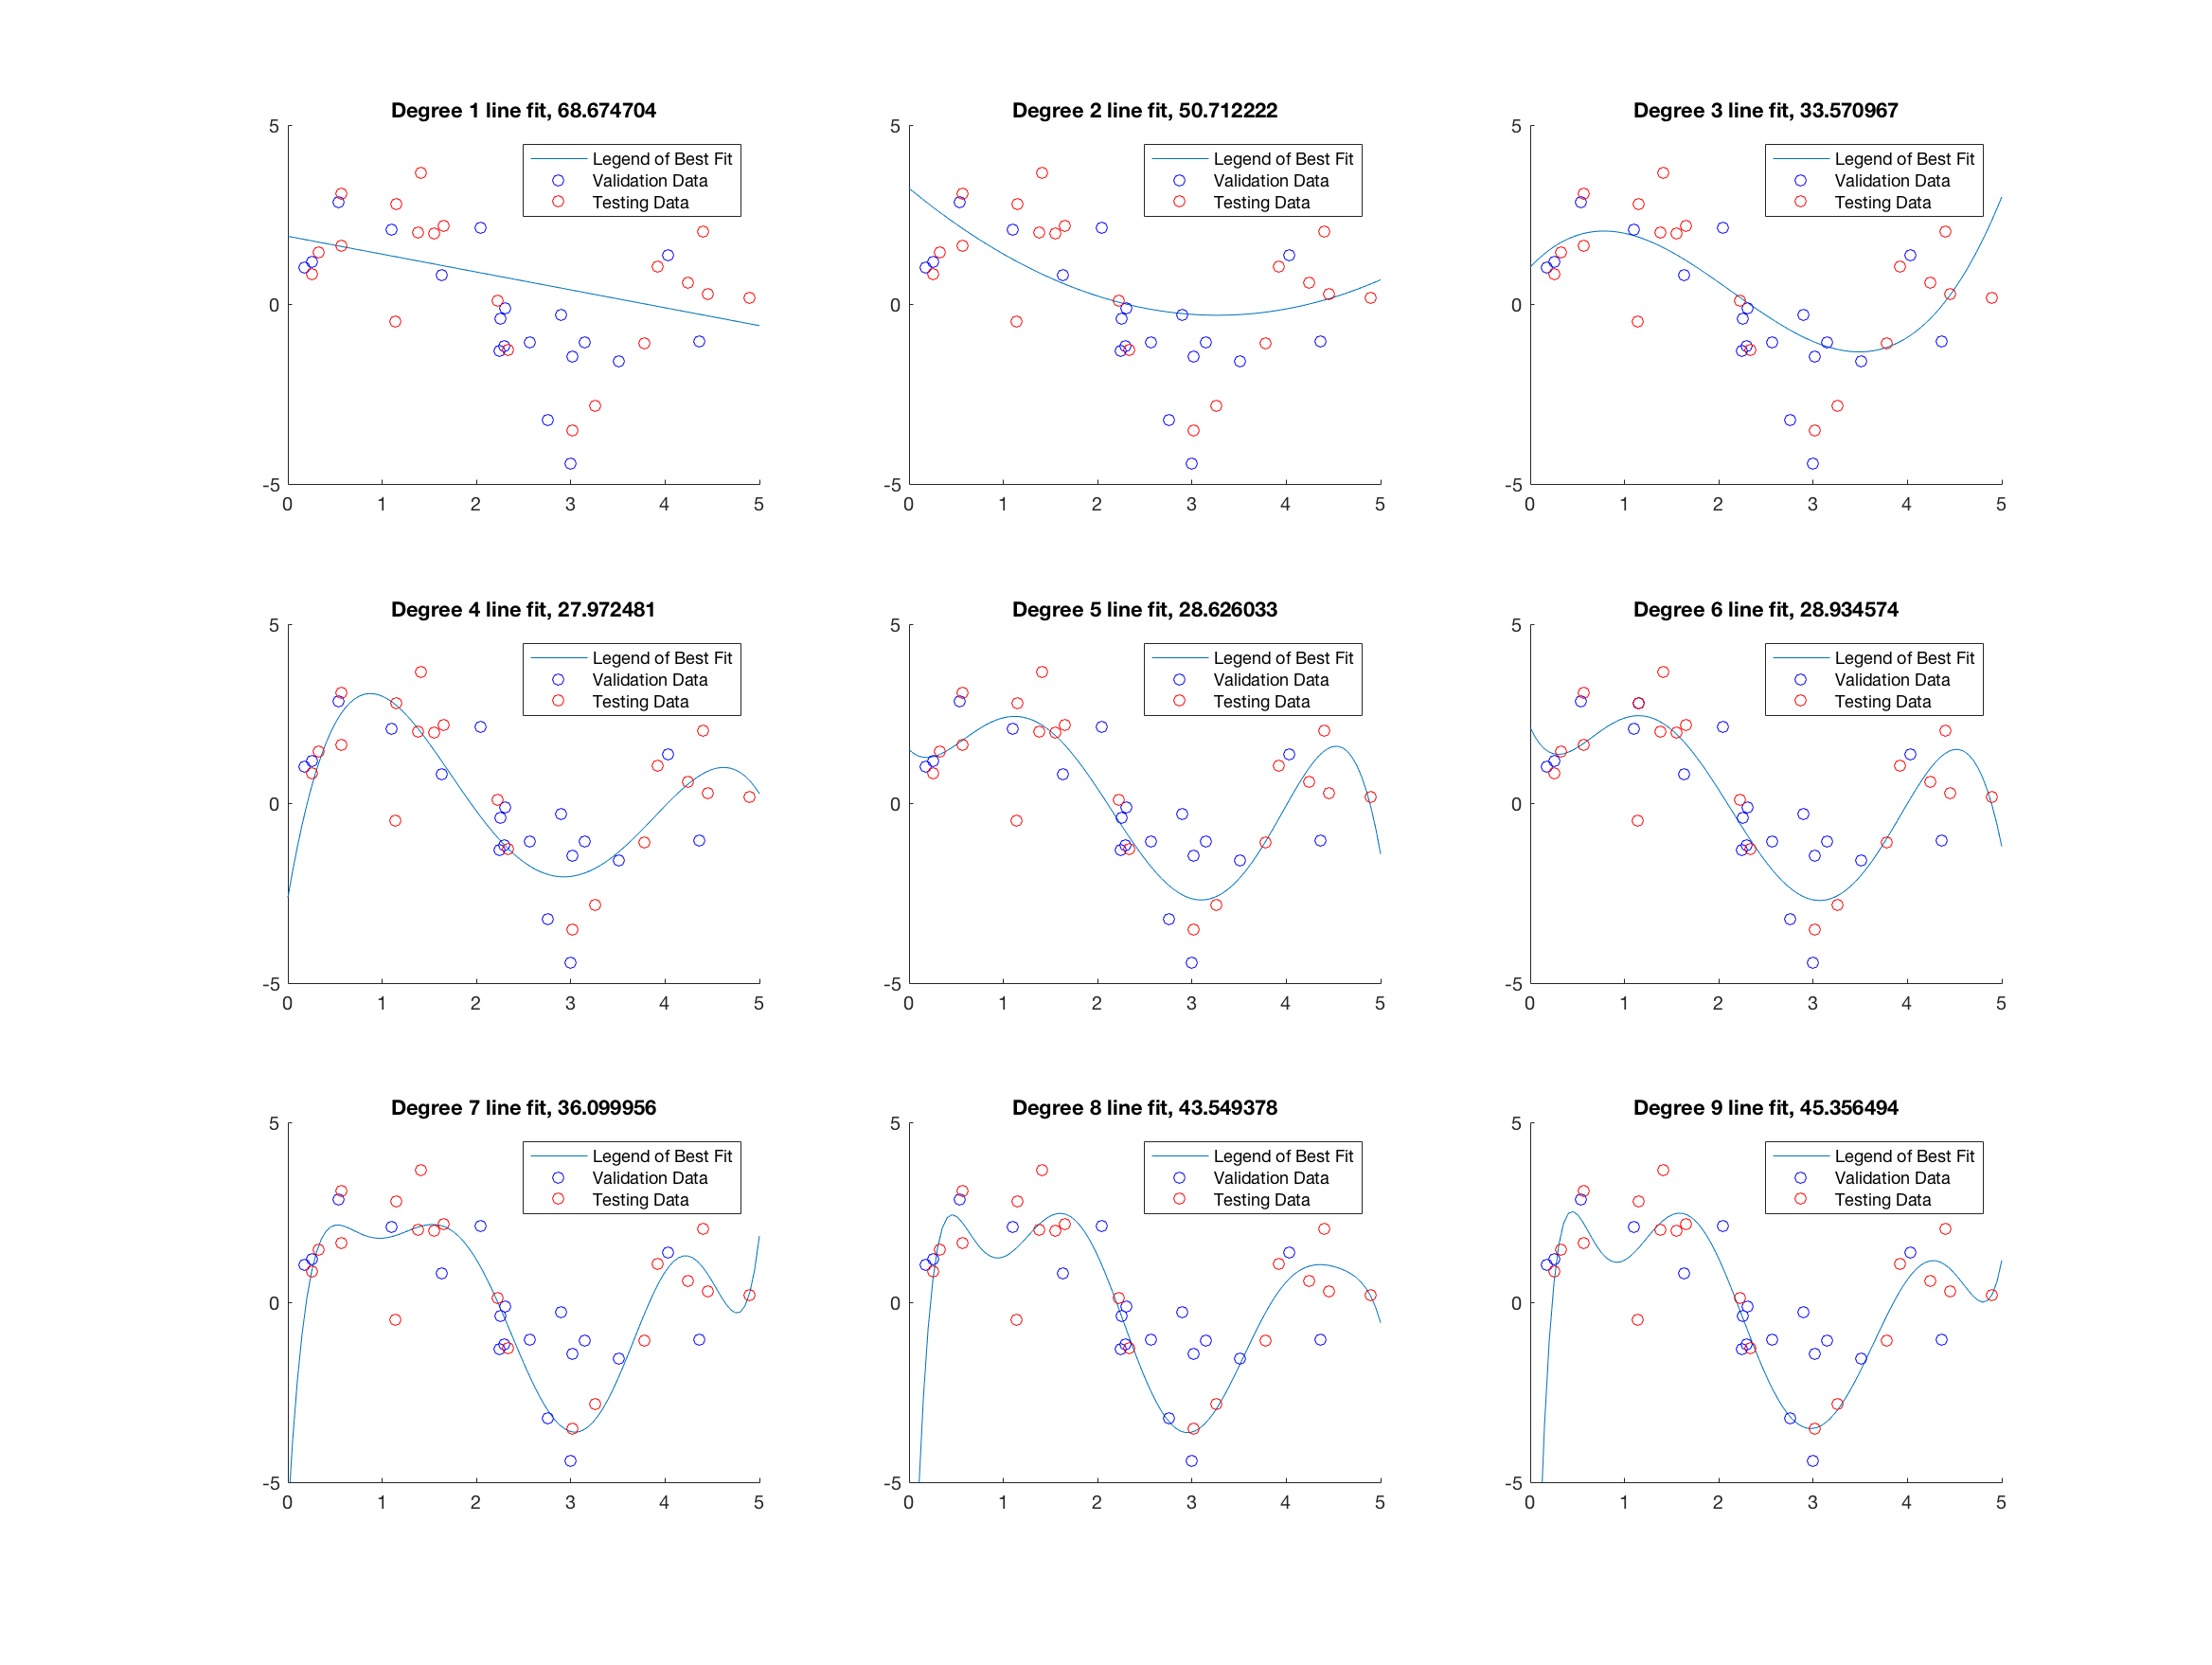
\includegraphics[width=\linewidth]{../../pracs/week3/images/q1_lines_of_best_fit}
    \centering
    \caption{Lines of best fit}
\end{figure}

\begin{figure}[H]
    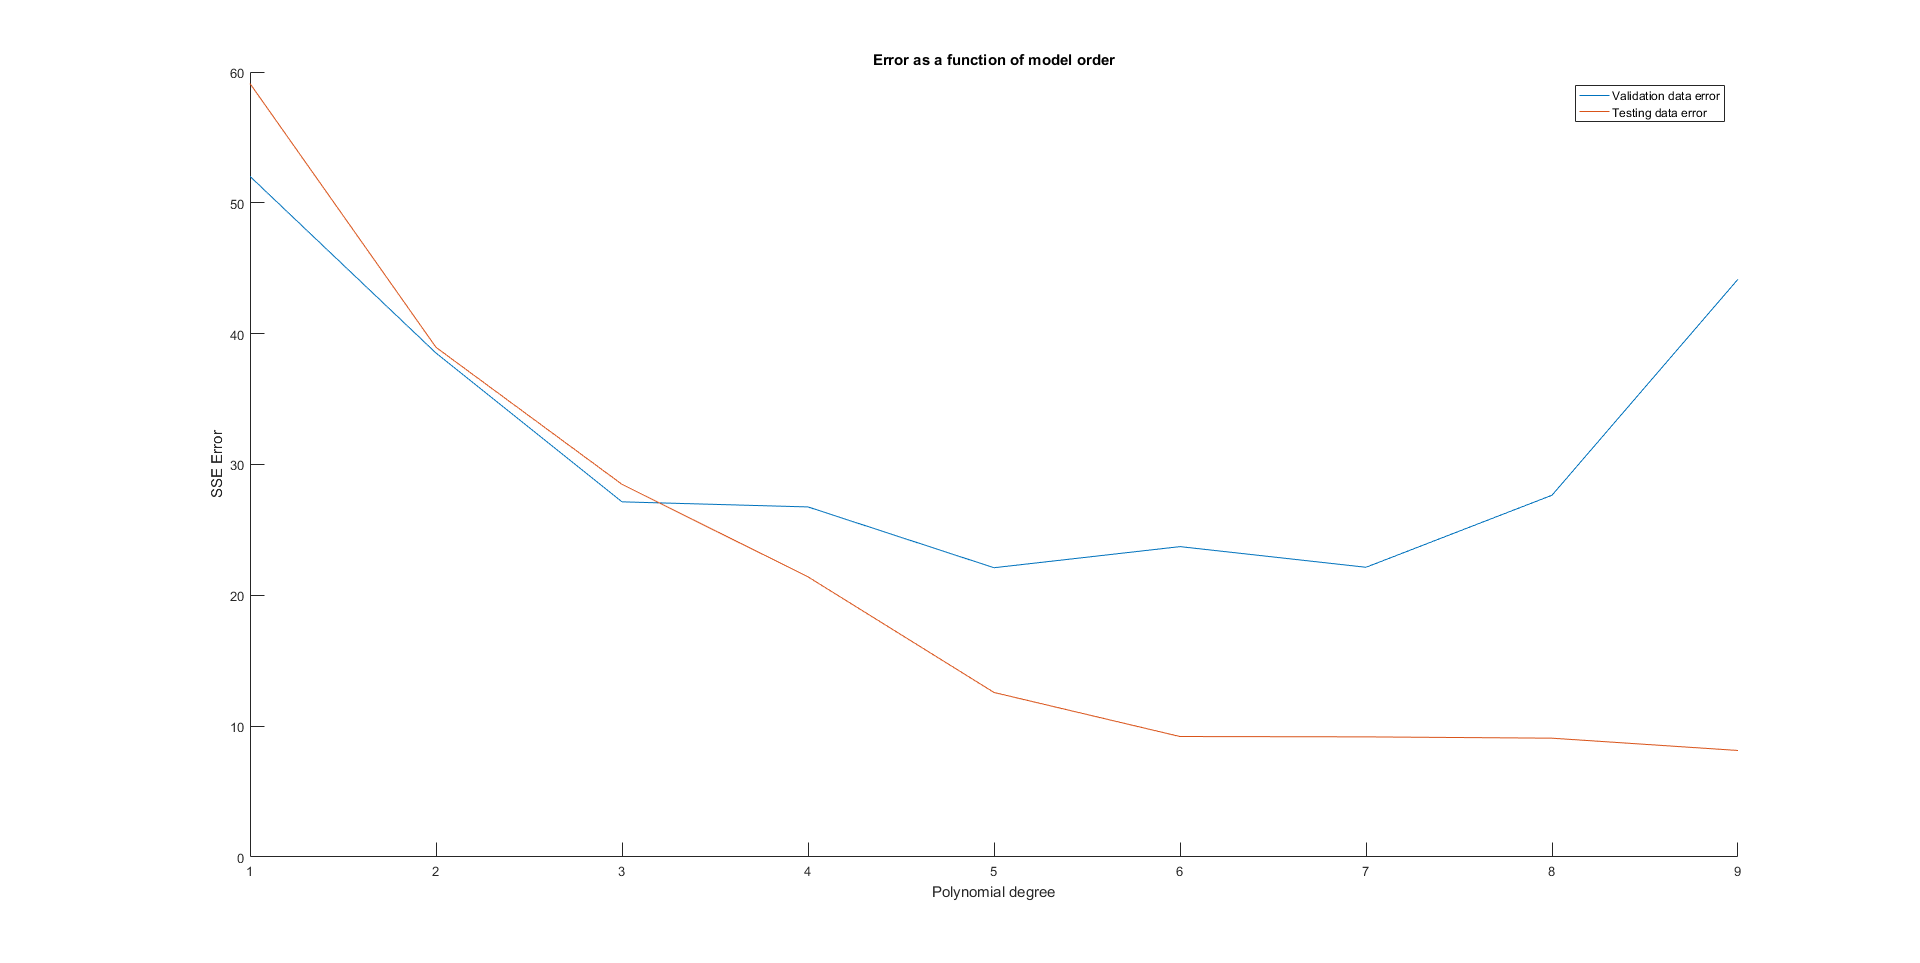
\includegraphics[width=\linewidth]{../../pracs/week3/images/q1_err_vs_degree}
    \centering
    \caption{Error vs Polynomial Degree}
\end{figure}

The above figure shows that as more polynomial degrees are introduced the error on the testing data decreases, which is expected as this was the data the model was trained on. However the error on the validation data increases after the 7th polynomial, thus we are overfitting the data.

\section*{Question 2.4}

\lstinputlisting[language=Matlab]{../../pracs/week3/q4.m}

\begin{figure}[H]
    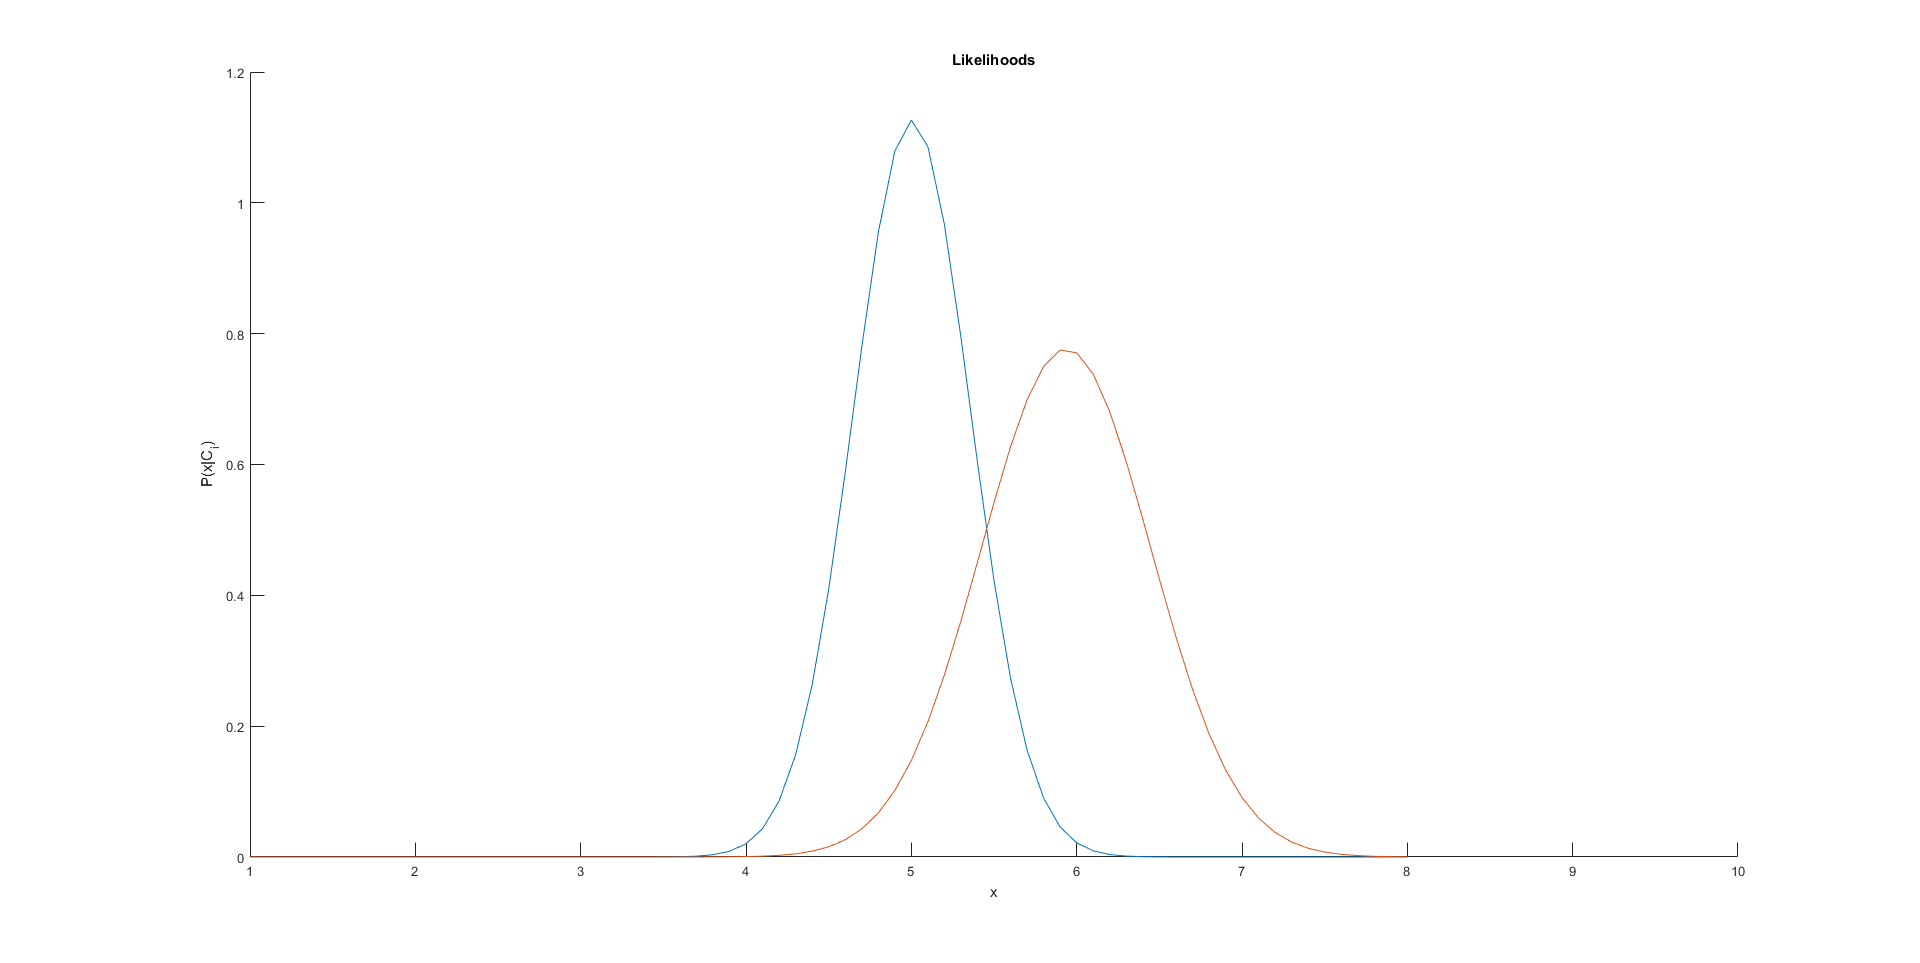
\includegraphics[width=\linewidth]{../../pracs/week3/images/q4_likelihoods}
    \centering
    \caption{Likelihoods}
\end{figure}

\begin{figure}[H]
    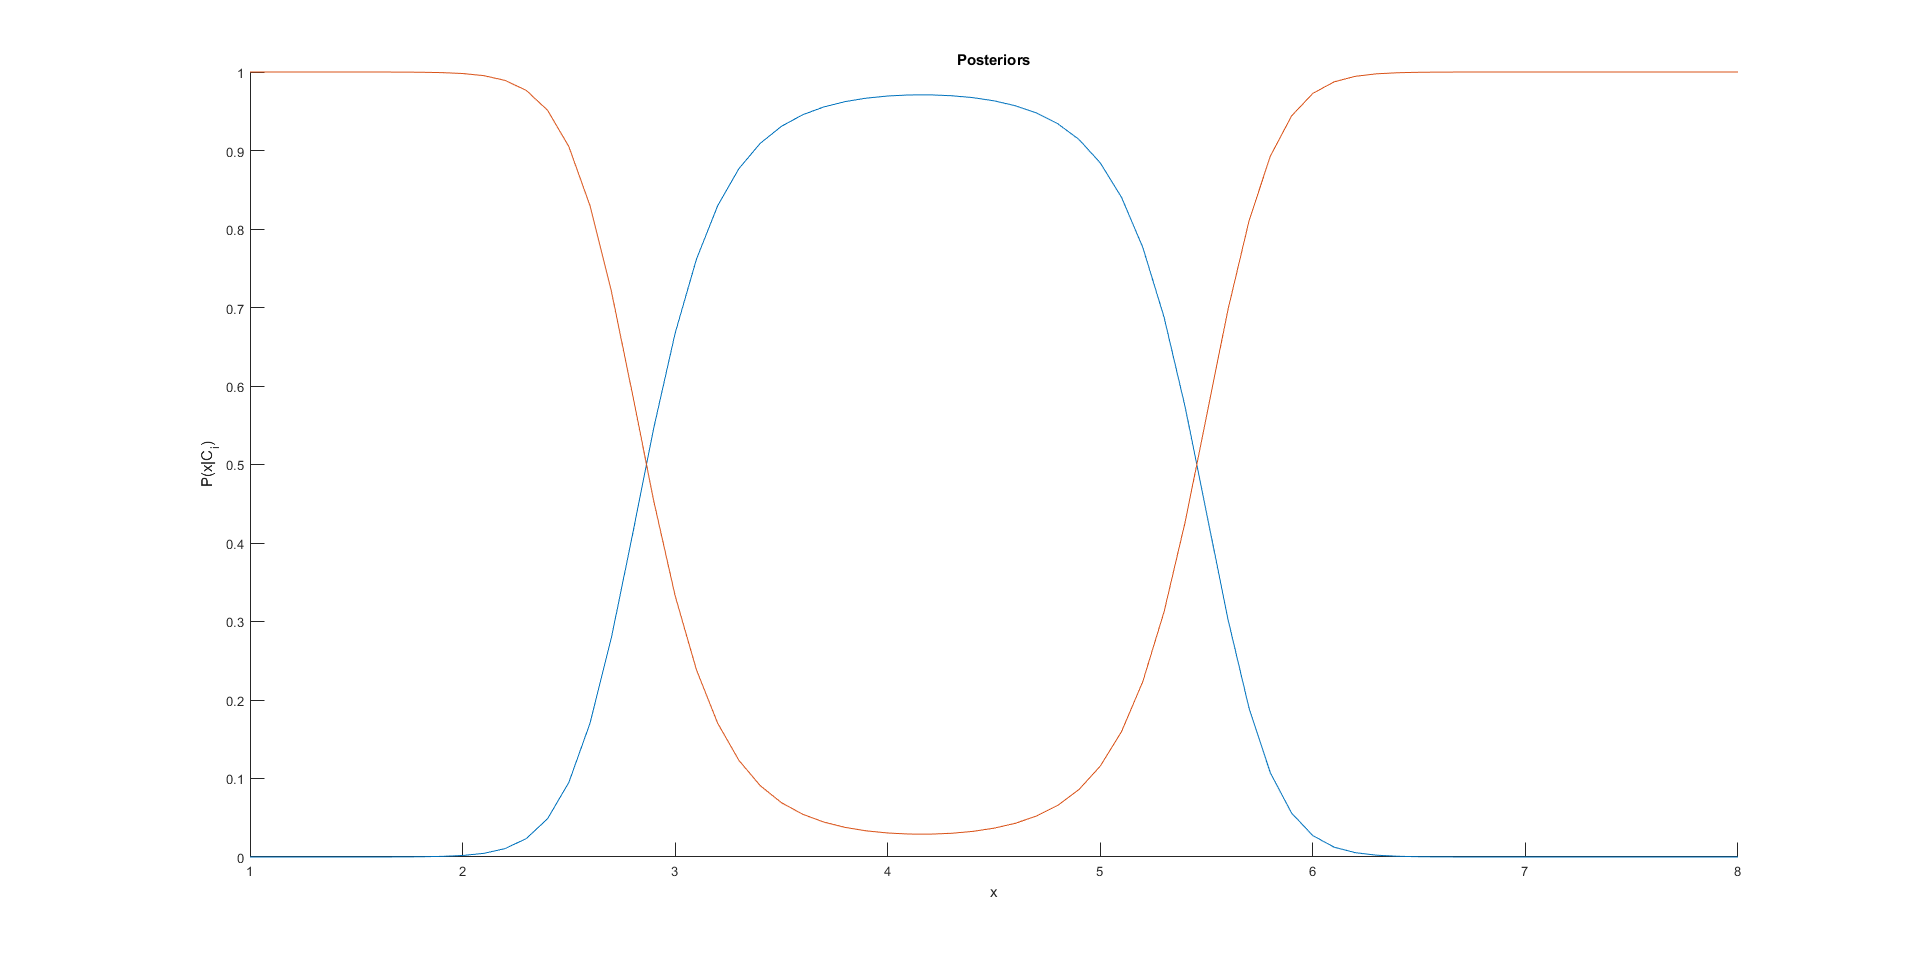
\includegraphics[width=\linewidth]{../../pracs/week3/images/q4_posteriors}
    \centering
    \caption{Posteriors}
\end{figure}

\section*{Question 3.1}

With the given dataset, we want to find a way to classify the two classes, this can be given by the posterior $P(C_i|x)$. To do so we first need to estimate the prior $P(C_i)$ and $p(x|C)$. This will allow us to estimate the proportion of data points for a given class $i$.  $p(x|c)$ can easily be found by using the matlab function \texttt{mvnpdf}.

Finding the posteriors for each class yields the below histogram.

\begin{figure}[H]
    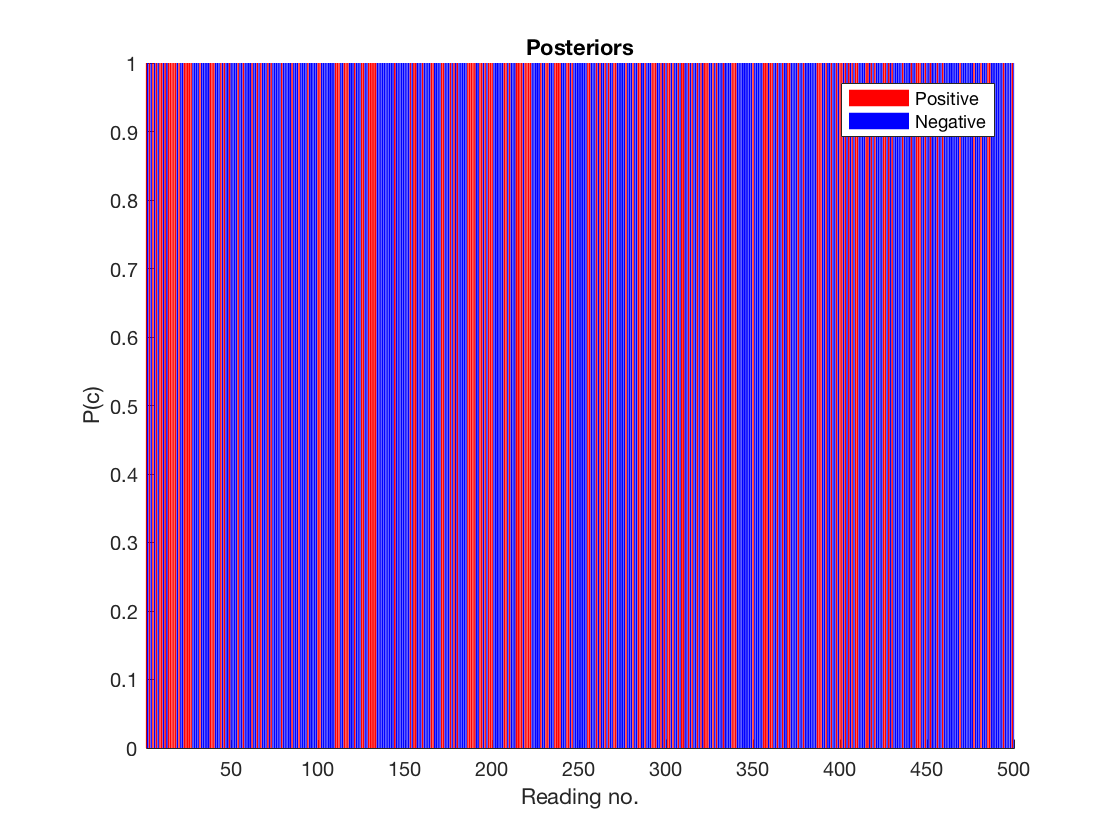
\includegraphics[width=\linewidth]{../../pracs/week4/images/q1_posteriors}
    \centering
    \caption{Posteriors}
\end{figure}

\section*{Question 3.2}

\section*{Question 3.5}

The computed KL values are listed in the table below
\begin{center}
    \begin{tabular}{|c|c|c|}
        \hline
        M and H1 & 2.6898 \\
        M and K1 & 0.2741  \\
        M and K2 & 0.28186 \\
        \hline
    \end{tabular}
\end{center}

There was an issue encountered while finding these variables, it was caused by the 0 values in some of the bins of the histogram estimator, this caused the division to produce Infinity values. This was fixed by replacing the infinity values with 0.

\begin{figure}[H]
    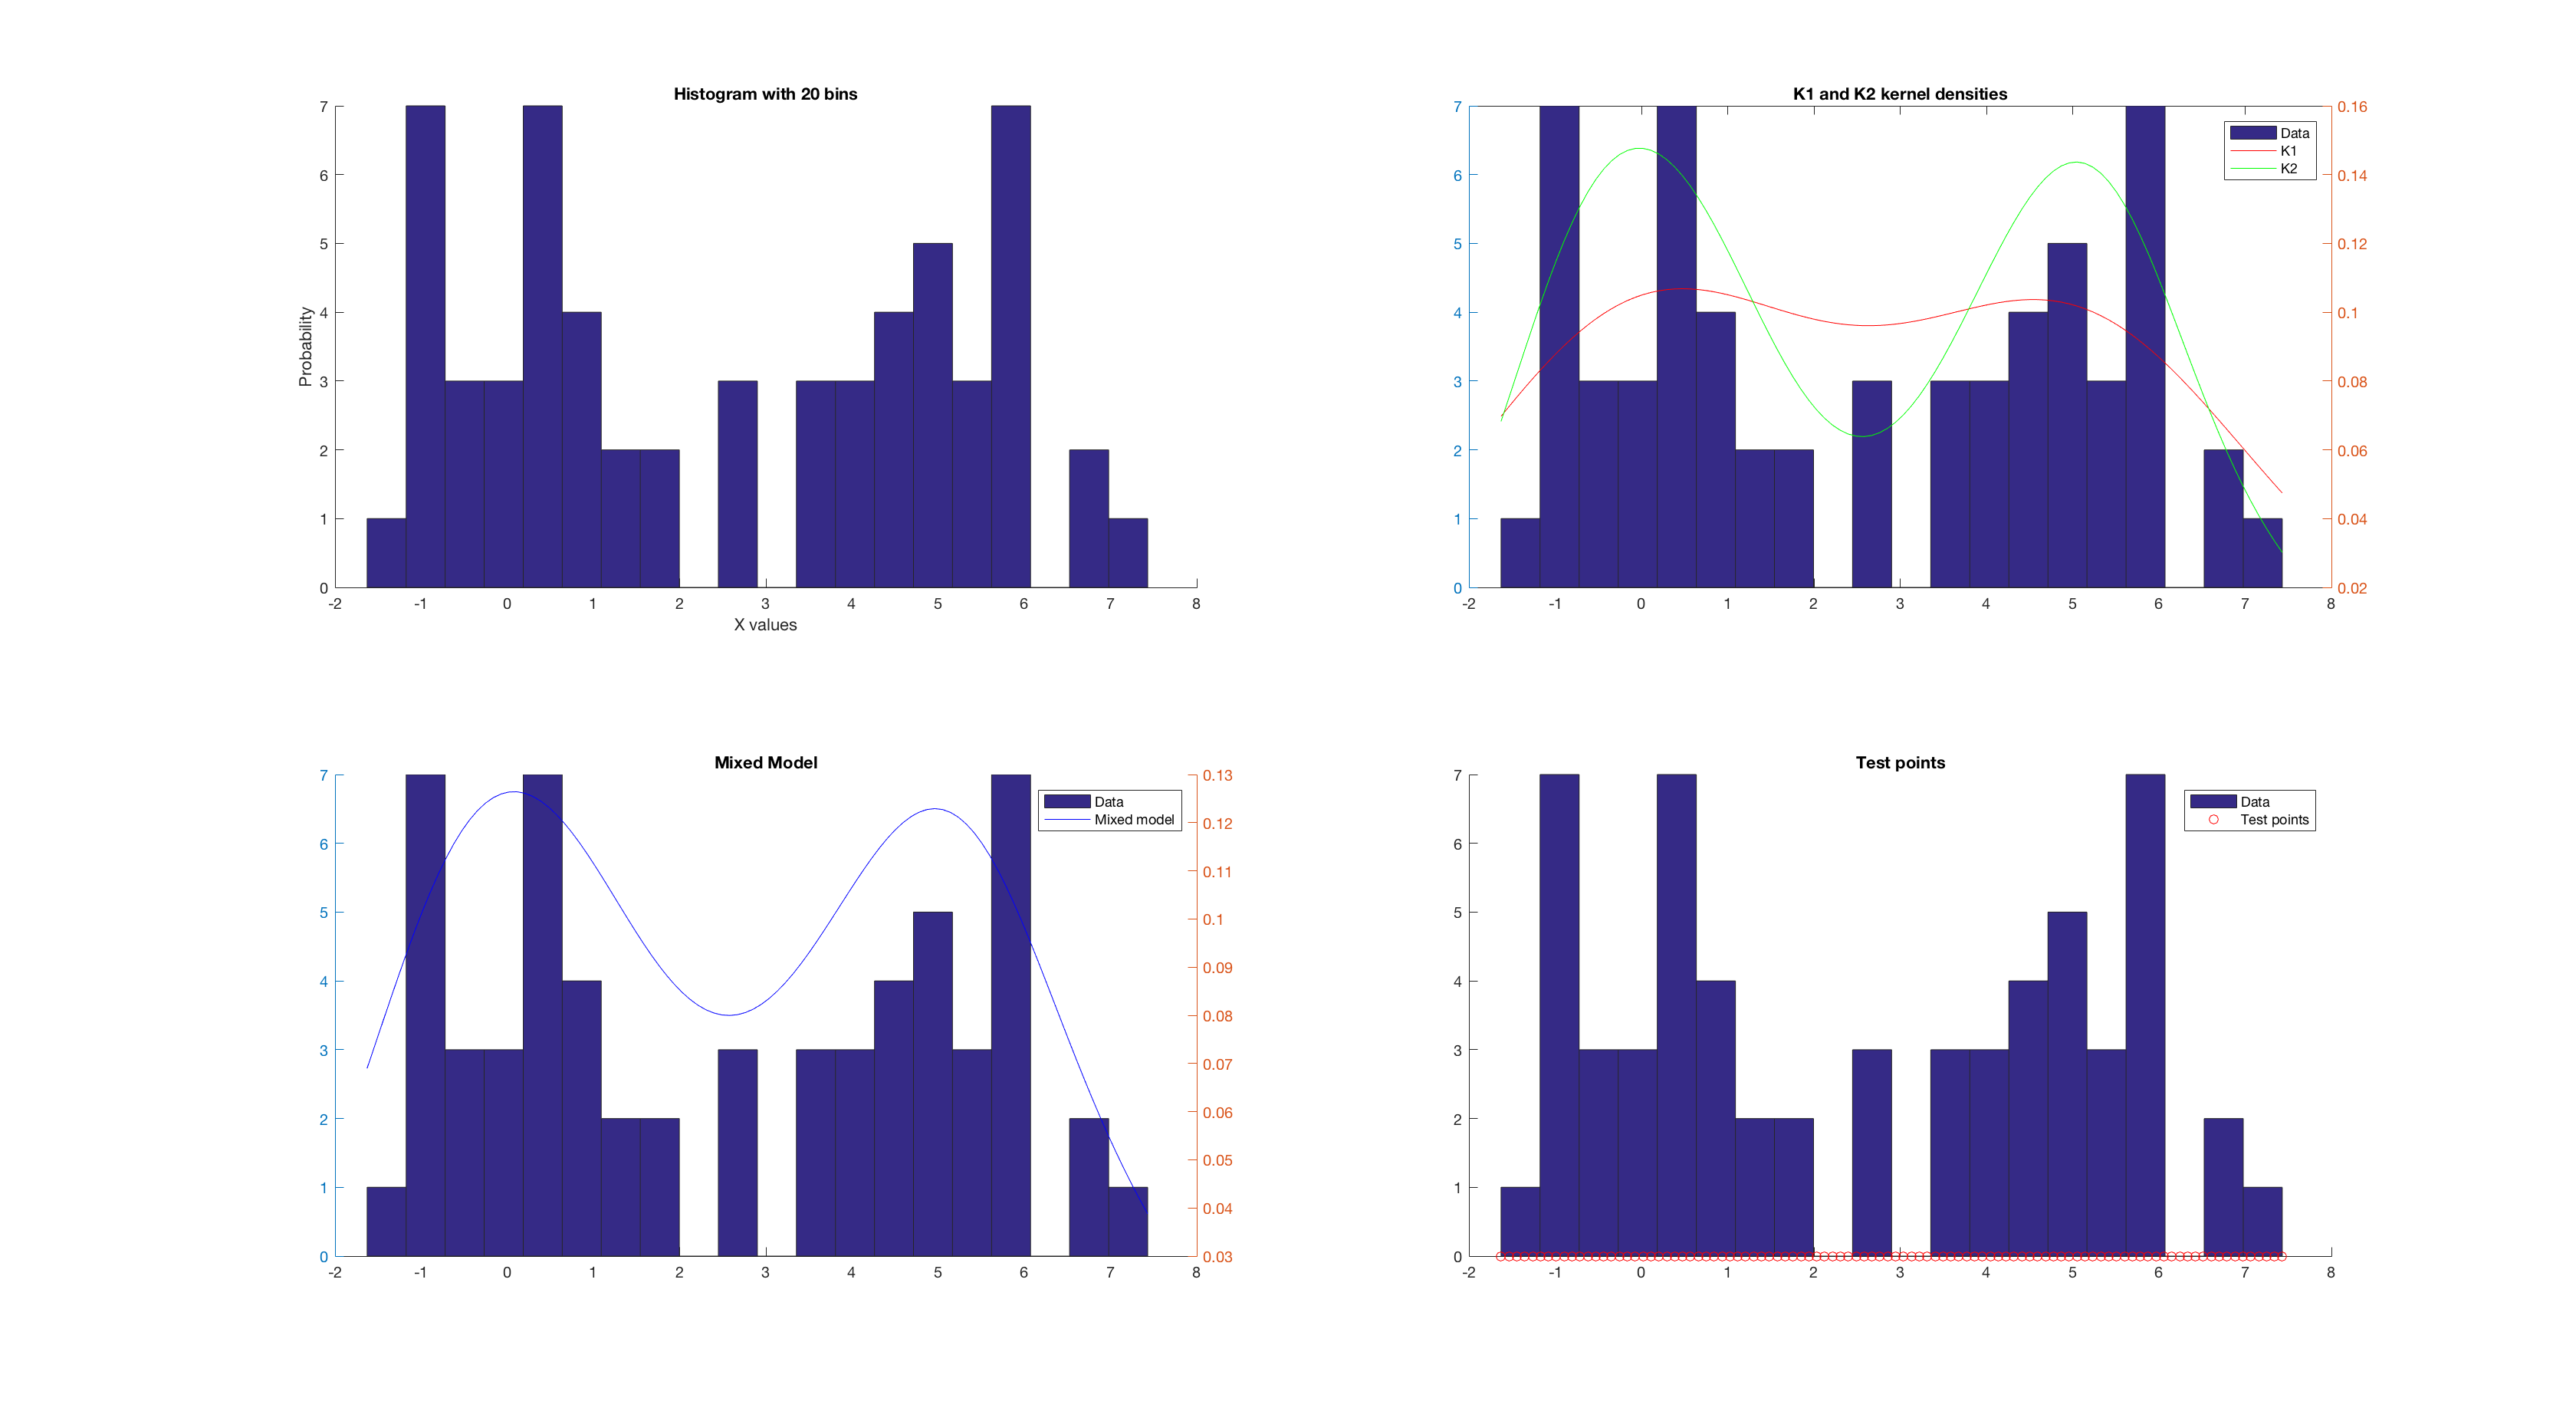
\includegraphics[width=\linewidth]{../../pracs/week4/images/q5}
    \centering
    \caption{Q5}
\end{figure}

Below is the code used to calculate the KL function, see the function called \texttt{KL} at the bottom of the script.

\lstinputlisting[language=Matlab]{../../pracs/week4/q5.m}

\end{document}
